\documentclass[aspectratio=169,t,xcolor=table]{beamer}
\usepackage[utf8]{inputenc}

\usepackage{booktabs} 
\usepackage{subcaption}

\usetheme{Ufg}
\setbeamertemplate{theorems}[numbered]
\setbeamertemplate{caption}[numbered]

\setPrimaryColor{UFGBlue} 
\usetikzlibrary{calc, shapes.geometric, arrows.meta, fit, positioning}

\begin{document}
\title[Inf UFG]{Assignment 9}
\subtitle{Technical Communication}

\author{ OneTouch: Effortless 2FA Scheme to Secure \\ Fingerprint Authentication with Wearable OTP Token}
\institute[UFG]
{
 \\ \\ \ \\ Utkarsh Kumar \\ 23114101 \\  \ \\
  Indian Institute of Technology\\
  Roorkee, Uttarakhand
}
\date{}
\setLogos{}
\frame[noframenumbering]{\titlepage}

\setLayout{vertical}
\begin{frame}
    \frametitle{Table of Contents}
    \tableofcontents
\end{frame}

\section{Motivation}
\setLayout{vertical}
\begin{frame}{Motivation}
    \begin{itemize}
        \item \textbf{Biometric Vulnerability:} Fingerprint authentication faces escalating threats from leaked databases and high-fidelity 3D-printed replicas.
        \item \textbf{The Liveness Detection Arms Race:} Software-based anti-spoofing is constantly bypassed by adaptive adversaries.
        \item \textbf{Friction of Traditional 2FA:} Conventional methods introduce significant interaction overhead, modifying the user habit.
        \item \textbf{Hardware Constraints:} Many deployed fingerprint devices completely lack the necessary I/O interfaces or reliable wireless modules required for standard 2FA.
        \item \textbf{Goal:} To implement an effortless, secure secondary authentication factor that operates natively through existing capacitive scanners via simple firmware updates.
    \end{itemize}
\end{frame}

\section{Problem Statement}
\begin{frame}{Problem statement}
    \begin{block}{Core Challenge}
        How can we integrate a strong authentication factor into existing fingerprint devices while preserving the effortless one-touch user experience and avoiding the requirement for hardware interfaces?
    \end{block}
    
    \vspace{1cm}
    \textbf{Design Requirements:}
    \begin{itemize}
        \item \textbf{Seamless Interaction Flow:} The user should simply press their finger onto the scanner, with no further manual data entry required.
        \item \textbf{Minimal Hardware Needs:} Maximize deployment compatibility by solely utilizing the built-in capacitive fingerprint scanner.
        \item \textbf{Enhanced Security:} Ensure the secondary communication medium acts to minimize potential interception risks.
    \end{itemize}
\end{frame}

\section{Proposed Architecture}
\setLayout{mainpoint}
\setBGColor{UFGBlue}
\begin{frame}
    \frametitle{Proposed Architecture}
\end{frame}

\setLayout{vertical}

\begin{frame}{OneTouch System Architecture}
\begin{figure}[h]
    \resizebox{0.8\textwidth}{!}{
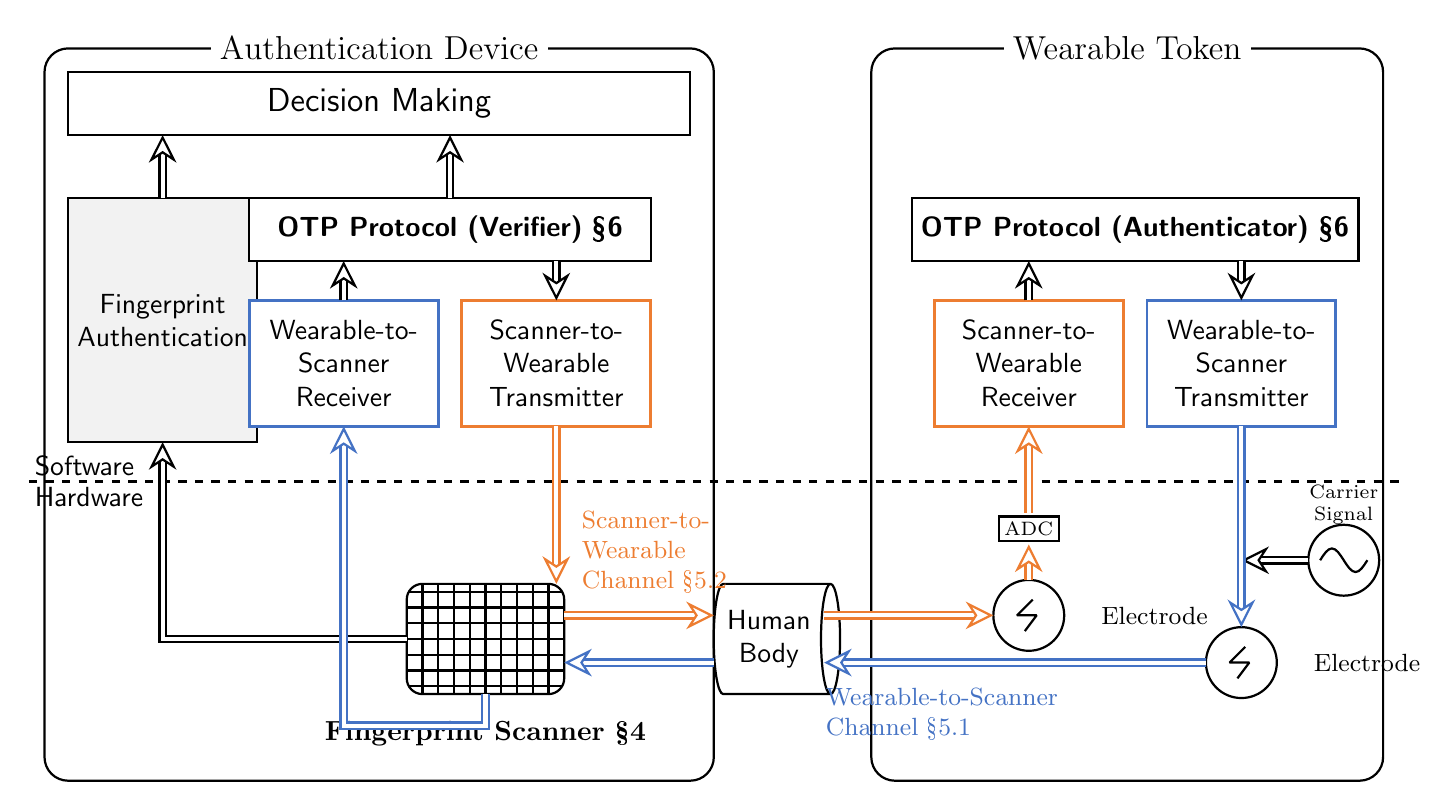
\begin{tikzpicture}[
    >=stealth,
    font=\sffamily,
    cblue/.style={color=mblu},
    corange/.style={color=morg},
    mblu/.style={RGB}{68,114,196},
    morg/.style={RGB}{237,125,49},
    box/.style={draw=black, thick, fill=white, align=center},
    bbox/.style={box, draw=mblu, line width=1pt},
    obox/.style={box, draw=morg, line width=1pt},
    fpbox/.style={box, fill=gray!10},
    darrow/.style={-{Stealth[length=3.5mm, width=3.5mm, fill=white]}, thick, draw=#1, double=white, double distance=1.5pt}
]

\definecolor{mblu}{RGB}{68,114,196}
\definecolor{morg}{RGB}{237,125,49}

\draw[dashed, thick] (-9.2, 0) -- (8.2, 0);
\node[anchor=south west, inner sep=2pt] at (-9.2, 0) {Software};
\node[anchor=north west, inner sep=2pt] at (-9.2, 0) {Hardware};

\draw[thick, rounded corners=3mm] (-9.0, -3.8) rectangle (-0.5, 5.5);
\node[fill=white, font=\large] at (-4.75, 5.5) {Authentication Device};
\draw[thick, rounded corners=3mm] (1.5, -3.8) rectangle (8.0, 5.5);
\node[fill=white, font=\large] at (4.75, 5.5) {Wearable Token};
\node[fpbox, minimum width=2.4cm, minimum height=3.1cm] (fp_auth) at (-7.5, 2.05) {Fingerprint\\Authentication};
\node[bbox, minimum width=2.4cm, minimum height=1.6cm] (ws_rec_auth) at (-5.2, 1.5) {Wearable-to-\\Scanner\\Receiver};
\node[obox, minimum width=2.4cm, minimum height=1.6cm] (sw_trans_auth) at (-2.5, 1.5) {Scanner-to-\\Wearable\\Transmitter};

\node[box, minimum width=5.1cm, minimum height=0.8cm] (otp_verif) at (-3.85, 3.2) {\textbf{OTP Protocol (Verifier) \S 6}};
\node[box, minimum width=7.9cm, minimum height=0.8cm] (decision) at (-4.75, 4.8) {\large Decision Making};
\node[draw, thick, rounded corners=2mm, minimum width=2.0cm, minimum height=1.4cm, fill=white] (scanner_bg) at (-3.4, -2.0) {};
\begin{scope}
    \clip[rounded corners=2mm] (-4.4, -2.7) rectangle (-2.4, -1.3);
    \draw[step=0.2cm, thick] (-4.5, -2.8) grid (-2.3, -1.2);
\end{scope}
\node[font=\bfseries] at (-3.4, -3.2) {Fingerprint Scanner \S 4};

\node[cylinder, draw, thick, shape border rotate=0, aspect=0.25, minimum height=1.6cm, minimum width=1.4cm, align=center, fill=white] (body) at (0.2, -2.0) {Human\\Body};
\node[obox, minimum width=2.4cm, minimum height=1.6cm] (sw_rec_token) at (3.5, 1.5) {Scanner-to-\\Wearable\\Receiver};
\node[bbox, minimum width=2.4cm, minimum height=1.6cm] (ws_trans_token) at (6.2, 1.5) {Wearable-to-\\Scanner\\Transmitter};
\node[box, minimum width=5.1cm, minimum height=0.8cm] (otp_auth) at (4.85, 3.2) {\textbf{OTP Protocol (Authenticator) \S 6}};
\node[draw, thick, circle, minimum size=0.9cm, fill=white] (elec_orange) at (3.5, -1.7) {};
\draw[thick, join=bevel] (3.55, -1.5) -- (3.35, -1.7) -- (3.6, -1.7) -- (3.45, -1.9);
\node[right=0.45cm of elec_orange, font=\small, inner sep=0pt] {Electrode};

\node[draw, thick, fill=white, inner sep=2pt, font=\scriptsize] (adc) at (3.5, -0.6) {ADC};
\node[draw, thick, circle, minimum size=0.9cm, fill=white] (elec_blue) at (6.2, -2.3) {};
\draw[thick, join=bevel] (6.25, -2.1) -- (6.05, -2.3) -- (6.3, -2.3) -- (6.15, -2.5);
\node[right=0.45cm of elec_blue, font=\small, inner sep=0pt] {Electrode};

\node[draw, thick, circle, minimum size=0.9cm, fill=white] (carrier) at (7.5, -1.0) {};
\draw[thick] (7.2, -1.0) sin (7.35, -0.85) cos (7.5, -1.0) sin (7.65, -1.15) cos (7.8, -1.0);
\node[font=\scriptsize, align=center] at (7.5, -0.3) {Carrier\\Signal};

\draw[darrow=black] (-7.5, 3.6) -- (-7.5, 4.4);
\draw[darrow=black] (-3.85, 3.6) -- (-3.85, 4.4);
\draw[darrow=black] (-5.2, 2.3) -- (-5.2, 2.8);
\draw[darrow=black] (-2.5, 2.8) -- (-2.5, 2.3);
\draw[darrow=black] (-4.4, -2.0) -| (-7.5, 0.5);
\draw[darrow=black] (3.5, 2.3) -- (3.5, 2.8);
\draw[darrow=black] (6.2, 2.8) -- (6.2, 2.3);
\draw[darrow=black] (7.05, -1.0) -- (6.2, -1.0);

\draw[darrow=morg] (-2.5, 0.7) -- (-2.5, -1.3);
\draw[darrow=morg] (-2.4, -1.7) -- (-0.5, -1.7);
\draw[darrow=morg] (0.9, -1.7) -- (3.05, -1.7);
\draw[darrow=morg] (3.5, -1.25) -- (3.5, -0.8); 
\draw[darrow=morg] (3.5, -0.4) -- (3.5, 0.7);

\node[text=morg, font=\small, align=left, anchor=west] at (-2.3, -0.9) {Scanner-to-\\Wearable\\Channel \S 5.2};
\draw[darrow=mblu] (6.2, 0.7) -- (6.2, -1.85);
\draw[darrow=mblu] (5.75, -2.3) -- (0.9, -2.3);
\draw[darrow=mblu] (-0.5, -2.3) -- (-2.4, -2.3);
\draw[darrow=mblu] (-3.4, -2.7) -- (-3.4, -3.1) -| (-5.2, 0.7);
\node[text=mblu, font=\small, align=left, anchor=north west] at (0.8, -2.5) {Wearable-to-Scanner\\Channel \S 5.1};

\end{tikzpicture}}
\caption{System Architecture\cite{onetouch}}
\end{figure}
\end{frame}

\begin{frame}{Architecture Details}
    \textbf{Establishing Touch-Based Channels:}
    \begin{itemize}
        \item \textbf{Wearable-to-Scanner (Uplink):} The wearable device causes the body to experience temporary changes in voltage levels. The capacitive scanner natively captures these changes line-by-line as it measures pixels.
        \item \textbf{Scanner-to-Wearable (Downlink):} The drive voltage emitted upon touch was varied by the scanner and this was determined with the help of an electrode kept in touch with the skin.
    \end{itemize}
    \vspace{0.5em}
    \textbf{Authentication Flow:}
    \begin{itemize}
        \item User physically touches the scanner.
        \item Primary factor - Scanner verifies fingerprint.
        \item Secondary factor - System invokes a Challenge-Response OTP exchange across the body.
        \item Access is granted only when both validations pass concurrently.
    \end{itemize}
\end{frame}

\section{Security threats}
\setLayout{vertical}
\begin{frame}{Security threats}
    \begin{itemize}
        \item \textbf{Fingerprint Spoofing:}The attackers are using physical entities (such as 3D-printed molds) for bypassing the initial biometric verification step.
        \item \textbf{Wireless Eavesdropping:} Electromagnetic signals escape the high-frequency body-based signal transmission and can be remotely detected.
        \item \textbf{In-Contact Relay Attack:} A highly skilled adversary bridges contact between the isolated wearable token and the authentication scanner to relay challenges.
        \item \textbf{Man in the Middle Attack:} The unauthenticated exchange of shared secrets could allow an hacker to intercept the setup phase.
        \item \textbf{Compromised Token Risks:} If an attacker manage to spoof a fingerprint and also steal the physical token, all systems might be bypassed.
    \end{itemize}
\end{frame}

\section{Analysis of Proposed Solution}
\setLayout{vertical}
\begin{frame}{Analysis of Proposed Solution}
\vspace{-1em}
    \begin{block}{Security Strengths of OneTouch}
        The secondary channel requires physical contact which prevents unauthorized access to the system. The system uses a unique OTP challenge-response mechanism which makes it resistant to replay attacks.
    \end{block}
    
    \vspace{1em}
    
    \textbf{Evaluating Mitigations:}
    \begin{itemize}
        \item \textbf{Relay Attacks:} The process of installing an in-contact relay system requires advanced coordination skills. The enforcement of strict distance and time limits establishes boundaries that restrict this particular vector.
        \item \textbf{MITM Setup:} Recommends pairing in trusted environments and adding strong device-bound certificates.
        \item \textbf{Brute Force \& Token Loss:} The use of a 3-byte one-time password system limits the maximum length of passwords in combination with rate limiting systems which prevent automated password guessing attempts.
    \end{itemize}
\end{frame}

\section{Conclusion}
\setLayout{horizontal}
\begin{frame}{Conclusions}
    \begin{itemize}
    \item OneTouch adds extra security to fingerprint login without changing how users use it.
    \item It uses existing fingerprint scanners, so no new hardware is needed.
    \item Touch is used to send secure data, linking the user’s touch and identity.
    \item Tests show it works well and improves security on many devices.
\end{itemize}
\vspace{1em}
\section{References}
\textbf{\Large References}
\begin{thebibliography}{9}

\bibitem{onetouch}
Y. Yan, Z. Yang,
"OneTouch: Effortless 2FA Scheme to Secure Fingerprint Authentication with Wearable OTP Token", 2025 [Online]. Available: https://www.usenix.org/conference/usenixsecurity25/presentation/yan-yihui
\end{thebibliography}
\end{frame}

\setLayout{blank}
\begin{frame}
    \centering
    \vspace{2cm}
    \textbf{\Huge Thank You}
    \ \\  \ \\ \ \\ 
    \textit{Suggestions} \ \\
    \text{utkarsh\_k@cs.iitr.ac.in}
    
    \vspace{1.5cm}
    \begin{figure}
        \centering
        
\includegraphics[height=2cm]{imgs/iitr.png}  
    \end{figure}
    
\end{frame}

\end{document}